\documentclass[twoside]{book}

% Packages required by doxygen
\usepackage{calc}
\usepackage{doxygen}
\usepackage{graphicx}
\usepackage[utf8]{inputenc}
\usepackage{makeidx}
\usepackage{multicol}
\usepackage{multirow}
\usepackage{textcomp}
\usepackage[table]{xcolor}

% Font selection
\usepackage[T1]{fontenc}
\usepackage{mathptmx}
\usepackage[scaled=.90]{helvet}
\usepackage{courier}
\usepackage{amssymb}
\usepackage{sectsty}
\renewcommand{\familydefault}{\sfdefault}
\allsectionsfont{%
  \fontseries{bc}\selectfont%
  \color{darkgray}%
}
\renewcommand{\DoxyLabelFont}{%
  \fontseries{bc}\selectfont%
  \color{darkgray}%
}

% Page & text layout
\usepackage{geometry}
\geometry{%
  a4paper,%
  top=2.5cm,%
  bottom=2.5cm,%
  left=2.5cm,%
  right=2.5cm%
}
\tolerance=750
\hfuzz=15pt
\hbadness=750
\setlength{\emergencystretch}{15pt}
\setlength{\parindent}{0cm}
\setlength{\parskip}{0.2cm}
\makeatletter
\renewcommand{\paragraph}{%
  \@startsection{paragraph}{4}{0ex}{-1.0ex}{1.0ex}{%
    \normalfont\normalsize\bfseries\SS@parafont%
  }%
}
\renewcommand{\subparagraph}{%
  \@startsection{subparagraph}{5}{0ex}{-1.0ex}{1.0ex}{%
    \normalfont\normalsize\bfseries\SS@subparafont%
  }%
}
\makeatother

% Headers & footers
\usepackage{fancyhdr}
\pagestyle{fancyplain}
\fancyhead[LE]{\fancyplain{}{\bfseries\thepage}}
\fancyhead[CE]{\fancyplain{}{}}
\fancyhead[RE]{\fancyplain{}{\bfseries\leftmark}}
\fancyhead[LO]{\fancyplain{}{\bfseries\rightmark}}
\fancyhead[CO]{\fancyplain{}{}}
\fancyhead[RO]{\fancyplain{}{\bfseries\thepage}}
\fancyfoot[LE]{\fancyplain{}{}}
\fancyfoot[CE]{\fancyplain{}{}}
\fancyfoot[RE]{\fancyplain{}{\bfseries\scriptsize Generated on Mon Feb 5 2018 18\-:59\-:11 for My Project by Doxygen }}
\fancyfoot[LO]{\fancyplain{}{\bfseries\scriptsize Generated on Mon Feb 5 2018 18\-:59\-:11 for My Project by Doxygen }}
\fancyfoot[CO]{\fancyplain{}{}}
\fancyfoot[RO]{\fancyplain{}{}}
\renewcommand{\footrulewidth}{0.4pt}
\renewcommand{\chaptermark}[1]{%
  \markboth{#1}{}%
}
\renewcommand{\sectionmark}[1]{%
  \markright{\thesection\ #1}%
}

% Indices & bibliography
\usepackage{natbib}
\usepackage[titles]{tocloft}
\setcounter{tocdepth}{3}
\setcounter{secnumdepth}{5}
\makeindex

% Hyperlinks (required, but should be loaded last)
\usepackage{ifpdf}
\ifpdf
  \usepackage[pdftex,pagebackref=true]{hyperref}
\else
  \usepackage[ps2pdf,pagebackref=true]{hyperref}
\fi
\hypersetup{%
  colorlinks=true,%
  linkcolor=blue,%
  citecolor=blue,%
  unicode%
}

% Custom commands
\newcommand{\clearemptydoublepage}{%
  \newpage{\pagestyle{empty}\cleardoublepage}%
}


%===== C O N T E N T S =====

\begin{document}

% Titlepage & ToC
\hypersetup{pageanchor=false}
\pagenumbering{roman}
\begin{titlepage}
\vspace*{7cm}
\begin{center}%
{\Large My Project }\\
\vspace*{1cm}
{\large Generated by Doxygen 1.8.6}\\
\vspace*{0.5cm}
{\small Mon Feb 5 2018 18:59:11}\\
\end{center}
\end{titlepage}
\clearemptydoublepage
\tableofcontents
\clearemptydoublepage
\pagenumbering{arabic}
\hypersetup{pageanchor=true}

%--- Begin generated contents ---
\chapter{Hierarchical Index}
\section{Class Hierarchy}
This inheritance list is sorted roughly, but not completely, alphabetically\-:\begin{DoxyCompactList}
\item \contentsline{section}{Document}{\pageref{class_document}}{}
\item \contentsline{section}{Graphic\-Editor}{\pageref{class_graphic_editor}}{}
\item \contentsline{section}{Graphic\-Element}{\pageref{class_graphic_element}}{}
\begin{DoxyCompactList}
\item \contentsline{section}{Line}{\pageref{class_line}}{}
\item \contentsline{section}{Square}{\pageref{class_square}}{}
\item \contentsline{section}{Triangle}{\pageref{class_triangle}}{}
\end{DoxyCompactList}
\end{DoxyCompactList}

\chapter{Class Index}
\section{Class List}
Here are the classes, structs, unions and interfaces with brief descriptions\-:\begin{DoxyCompactList}
\item\contentsline{section}{\hyperlink{class_document}{Document} }{\pageref{class_document}}{}
\item\contentsline{section}{\hyperlink{class_graphic_editor}{Graphic\-Editor} }{\pageref{class_graphic_editor}}{}
\item\contentsline{section}{\hyperlink{class_graphic_element}{Graphic\-Element} }{\pageref{class_graphic_element}}{}
\item\contentsline{section}{\hyperlink{class_line}{Line} }{\pageref{class_line}}{}
\item\contentsline{section}{\hyperlink{class_square}{Square} }{\pageref{class_square}}{}
\item\contentsline{section}{\hyperlink{class_triangle}{Triangle} }{\pageref{class_triangle}}{}
\end{DoxyCompactList}

\chapter{File Index}
\section{File List}
Here is a list of all files with brief descriptions\-:\begin{DoxyCompactList}
\item\contentsline{section}{\hyperlink{header_8h}{header.\-h} }{\pageref{header_8h}}{}
\item\contentsline{section}{\hyperlink{main_8cpp}{main.\-cpp} }{\pageref{main_8cpp}}{}
\item\contentsline{section}{\hyperlink{version_8h}{version.\-h} }{\pageref{version_8h}}{}
\end{DoxyCompactList}

\chapter{Class Documentation}
\hypertarget{class_document}{\section{Document Class Reference}
\label{class_document}\index{Document@{Document}}
}


{\ttfamily \#include $<$header.\-h$>$}

\subsection*{Public Member Functions}
\begin{DoxyCompactItemize}
\item 
\hyperlink{class_document_acdbcbe550084e8c20f4f67eb229ad66a}{Document} ()
\item 
\hyperlink{class_document_aa8e412e814bf882e1e83782cbc2b0863}{Document} (const std\-::string \&filename)
\item 
void \hyperlink{class_document_ada3e03e1944b6473fe81077b8aa7479b}{export\-In\-File} (const std\-::string \&filename)
\item 
void \hyperlink{class_document_ab98b6d53b438a250cad4c999dd2e05cc}{create\-Element} (\hyperlink{class_graphic_element}{Graphic\-Element} $\ast$element)
\item 
void \hyperlink{class_document_addfac261c3fa23d7c03576c472e1ce7a}{remove\-Element} (\hyperlink{class_graphic_element}{Graphic\-Element} $\ast$element)
\end{DoxyCompactItemize}


\subsection{Constructor \& Destructor Documentation}
\hypertarget{class_document_acdbcbe550084e8c20f4f67eb229ad66a}{\index{Document@{Document}!Document@{Document}}
\index{Document@{Document}!Document@{Document}}
\subsubsection[{Document}]{\setlength{\rightskip}{0pt plus 5cm}Document\-::\-Document (
\begin{DoxyParamCaption}
{}
\end{DoxyParamCaption}
)\hspace{0.3cm}{\ttfamily [inline]}, {\ttfamily [explicit]}}}\label{class_document_acdbcbe550084e8c20f4f67eb229ad66a}
\hypertarget{class_document_aa8e412e814bf882e1e83782cbc2b0863}{\index{Document@{Document}!Document@{Document}}
\index{Document@{Document}!Document@{Document}}
\subsubsection[{Document}]{\setlength{\rightskip}{0pt plus 5cm}Document\-::\-Document (
\begin{DoxyParamCaption}
\item[{const std\-::string \&}]{filename}
\end{DoxyParamCaption}
)\hspace{0.3cm}{\ttfamily [inline]}, {\ttfamily [explicit]}}}\label{class_document_aa8e412e814bf882e1e83782cbc2b0863}


\subsection{Member Function Documentation}
\hypertarget{class_document_ab98b6d53b438a250cad4c999dd2e05cc}{\index{Document@{Document}!create\-Element@{create\-Element}}
\index{create\-Element@{create\-Element}!Document@{Document}}
\subsubsection[{create\-Element}]{\setlength{\rightskip}{0pt plus 5cm}void Document\-::create\-Element (
\begin{DoxyParamCaption}
\item[{{\bf Graphic\-Element} $\ast$}]{element}
\end{DoxyParamCaption}
)\hspace{0.3cm}{\ttfamily [inline]}}}\label{class_document_ab98b6d53b438a250cad4c999dd2e05cc}
\hypertarget{class_document_ada3e03e1944b6473fe81077b8aa7479b}{\index{Document@{Document}!export\-In\-File@{export\-In\-File}}
\index{export\-In\-File@{export\-In\-File}!Document@{Document}}
\subsubsection[{export\-In\-File}]{\setlength{\rightskip}{0pt plus 5cm}void Document\-::export\-In\-File (
\begin{DoxyParamCaption}
\item[{const std\-::string \&}]{filename}
\end{DoxyParamCaption}
)\hspace{0.3cm}{\ttfamily [inline]}}}\label{class_document_ada3e03e1944b6473fe81077b8aa7479b}
\hypertarget{class_document_addfac261c3fa23d7c03576c472e1ce7a}{\index{Document@{Document}!remove\-Element@{remove\-Element}}
\index{remove\-Element@{remove\-Element}!Document@{Document}}
\subsubsection[{remove\-Element}]{\setlength{\rightskip}{0pt plus 5cm}void Document\-::remove\-Element (
\begin{DoxyParamCaption}
\item[{{\bf Graphic\-Element} $\ast$}]{element}
\end{DoxyParamCaption}
)\hspace{0.3cm}{\ttfamily [inline]}}}\label{class_document_addfac261c3fa23d7c03576c472e1ce7a}


The documentation for this class was generated from the following file\-:\begin{DoxyCompactItemize}
\item 
\hyperlink{header_8h}{header.\-h}\end{DoxyCompactItemize}

\hypertarget{class_graphic_editor}{\section{Graphic\-Editor Class Reference}
\label{class_graphic_editor}\index{Graphic\-Editor@{Graphic\-Editor}}
}
\subsection*{Public Member Functions}
\begin{DoxyCompactItemize}
\item 
void \hyperlink{class_graphic_editor_a2a9ae27cefa241552c07bdbe39c8137b}{create\-Document} ()
\item 
void \hyperlink{class_graphic_editor_ad6cdff6bb334234610633529cb1e42f3}{import\-Document} (const std\-::string \&filename)
\item 
void \hyperlink{class_graphic_editor_a343385644b2f62c677285758f96086b3}{export\-Document} (const std\-::string \&filename)
\item 
void \hyperlink{class_graphic_editor_afc79eea9f8377959bc8be03d992be780}{add\-Element} (\hyperlink{class_graphic_element}{Graphic\-Element} $\ast$element)
\item 
void \hyperlink{class_graphic_editor_a27150d582800a620ada5e0c42f6dba43}{remove\-Element} (\hyperlink{class_graphic_element}{Graphic\-Element} $\ast$element)
\end{DoxyCompactItemize}


\subsection{Member Function Documentation}
\hypertarget{class_graphic_editor_afc79eea9f8377959bc8be03d992be780}{\index{Graphic\-Editor@{Graphic\-Editor}!add\-Element@{add\-Element}}
\index{add\-Element@{add\-Element}!GraphicEditor@{Graphic\-Editor}}
\subsubsection[{add\-Element}]{\setlength{\rightskip}{0pt plus 5cm}void Graphic\-Editor\-::add\-Element (
\begin{DoxyParamCaption}
\item[{{\bf Graphic\-Element} $\ast$}]{element}
\end{DoxyParamCaption}
)\hspace{0.3cm}{\ttfamily [inline]}}}\label{class_graphic_editor_afc79eea9f8377959bc8be03d992be780}
\hypertarget{class_graphic_editor_a2a9ae27cefa241552c07bdbe39c8137b}{\index{Graphic\-Editor@{Graphic\-Editor}!create\-Document@{create\-Document}}
\index{create\-Document@{create\-Document}!GraphicEditor@{Graphic\-Editor}}
\subsubsection[{create\-Document}]{\setlength{\rightskip}{0pt plus 5cm}void Graphic\-Editor\-::create\-Document (
\begin{DoxyParamCaption}
{}
\end{DoxyParamCaption}
)\hspace{0.3cm}{\ttfamily [inline]}}}\label{class_graphic_editor_a2a9ae27cefa241552c07bdbe39c8137b}
\hypertarget{class_graphic_editor_a343385644b2f62c677285758f96086b3}{\index{Graphic\-Editor@{Graphic\-Editor}!export\-Document@{export\-Document}}
\index{export\-Document@{export\-Document}!GraphicEditor@{Graphic\-Editor}}
\subsubsection[{export\-Document}]{\setlength{\rightskip}{0pt plus 5cm}void Graphic\-Editor\-::export\-Document (
\begin{DoxyParamCaption}
\item[{const std\-::string \&}]{filename}
\end{DoxyParamCaption}
)\hspace{0.3cm}{\ttfamily [inline]}}}\label{class_graphic_editor_a343385644b2f62c677285758f96086b3}
\hypertarget{class_graphic_editor_ad6cdff6bb334234610633529cb1e42f3}{\index{Graphic\-Editor@{Graphic\-Editor}!import\-Document@{import\-Document}}
\index{import\-Document@{import\-Document}!GraphicEditor@{Graphic\-Editor}}
\subsubsection[{import\-Document}]{\setlength{\rightskip}{0pt plus 5cm}void Graphic\-Editor\-::import\-Document (
\begin{DoxyParamCaption}
\item[{const std\-::string \&}]{filename}
\end{DoxyParamCaption}
)\hspace{0.3cm}{\ttfamily [inline]}}}\label{class_graphic_editor_ad6cdff6bb334234610633529cb1e42f3}
\hypertarget{class_graphic_editor_a27150d582800a620ada5e0c42f6dba43}{\index{Graphic\-Editor@{Graphic\-Editor}!remove\-Element@{remove\-Element}}
\index{remove\-Element@{remove\-Element}!GraphicEditor@{Graphic\-Editor}}
\subsubsection[{remove\-Element}]{\setlength{\rightskip}{0pt plus 5cm}void Graphic\-Editor\-::remove\-Element (
\begin{DoxyParamCaption}
\item[{{\bf Graphic\-Element} $\ast$}]{element}
\end{DoxyParamCaption}
)\hspace{0.3cm}{\ttfamily [inline]}}}\label{class_graphic_editor_a27150d582800a620ada5e0c42f6dba43}


The documentation for this class was generated from the following file\-:\begin{DoxyCompactItemize}
\item 
\hyperlink{main_8cpp}{main.\-cpp}\end{DoxyCompactItemize}

\hypertarget{class_graphic_element}{\section{Graphic\-Element Class Reference}
\label{class_graphic_element}\index{Graphic\-Element@{Graphic\-Element}}
}


{\ttfamily \#include $<$header.\-h$>$}



Inheritance diagram for Graphic\-Element\-:
\nopagebreak
\begin{figure}[H]
\begin{center}
\leavevmode
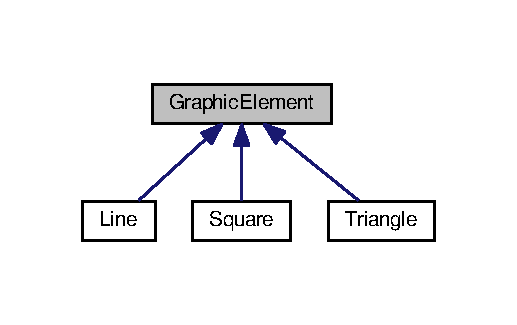
\includegraphics[width=248pt]{class_graphic_element__inherit__graph}
\end{center}
\end{figure}
\subsection*{Public Member Functions}
\begin{DoxyCompactItemize}
\item 
virtual void \hyperlink{class_graphic_element_ac059a330ae2aa071b80d4fc16f505a53}{create} ()=0
\item 
virtual void \hyperlink{class_graphic_element_a008cda41b56bfd1607067e478488405c}{remove} ()=0
\end{DoxyCompactItemize}


\subsection{Member Function Documentation}
\hypertarget{class_graphic_element_ac059a330ae2aa071b80d4fc16f505a53}{\index{Graphic\-Element@{Graphic\-Element}!create@{create}}
\index{create@{create}!GraphicElement@{Graphic\-Element}}
\subsubsection[{create}]{\setlength{\rightskip}{0pt plus 5cm}virtual void Graphic\-Element\-::create (
\begin{DoxyParamCaption}
{}
\end{DoxyParamCaption}
)\hspace{0.3cm}{\ttfamily [pure virtual]}}}\label{class_graphic_element_ac059a330ae2aa071b80d4fc16f505a53}


Implemented in \hyperlink{class_triangle_a13b75277f5c2cd4991b599657b02692e}{Triangle}, \hyperlink{class_square_a8f288729441c986e6fc37593c9c5346b}{Square}, and \hyperlink{class_line_ae7fc21dbce8b1c64ac4f44833c47ee9b}{Line}.

\hypertarget{class_graphic_element_a008cda41b56bfd1607067e478488405c}{\index{Graphic\-Element@{Graphic\-Element}!remove@{remove}}
\index{remove@{remove}!GraphicElement@{Graphic\-Element}}
\subsubsection[{remove}]{\setlength{\rightskip}{0pt plus 5cm}virtual void Graphic\-Element\-::remove (
\begin{DoxyParamCaption}
{}
\end{DoxyParamCaption}
)\hspace{0.3cm}{\ttfamily [pure virtual]}}}\label{class_graphic_element_a008cda41b56bfd1607067e478488405c}


Implemented in \hyperlink{class_triangle_a38c4f7a80a0ef3dda7bc90652b510b46}{Triangle}, \hyperlink{class_square_a90cb952f7266720cbd63513cd34a6fc3}{Square}, and \hyperlink{class_line_a946bc175a8015e7e083450a6b5efc107}{Line}.



The documentation for this class was generated from the following file\-:\begin{DoxyCompactItemize}
\item 
\hyperlink{header_8h}{header.\-h}\end{DoxyCompactItemize}

\hypertarget{class_line}{\section{Line Class Reference}
\label{class_line}\index{Line@{Line}}
}


{\ttfamily \#include $<$header.\-h$>$}



Inheritance diagram for Line\-:
\nopagebreak
\begin{figure}[H]
\begin{center}
\leavevmode
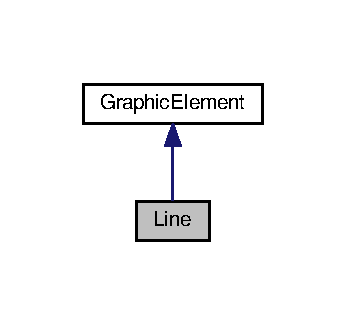
\includegraphics[width=166pt]{class_line__inherit__graph}
\end{center}
\end{figure}


Collaboration diagram for Line\-:
\nopagebreak
\begin{figure}[H]
\begin{center}
\leavevmode
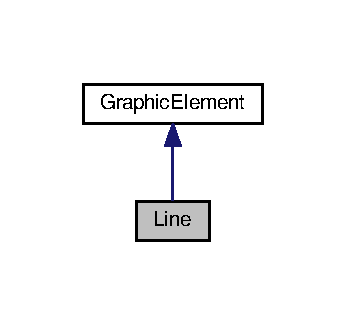
\includegraphics[width=166pt]{class_line__coll__graph}
\end{center}
\end{figure}
\subsection*{Public Member Functions}
\begin{DoxyCompactItemize}
\item 
void \hyperlink{class_line_ae7fc21dbce8b1c64ac4f44833c47ee9b}{create} () override
\item 
void \hyperlink{class_line_a946bc175a8015e7e083450a6b5efc107}{remove} () override
\end{DoxyCompactItemize}


\subsection{Member Function Documentation}
\hypertarget{class_line_ae7fc21dbce8b1c64ac4f44833c47ee9b}{\index{Line@{Line}!create@{create}}
\index{create@{create}!Line@{Line}}
\subsubsection[{create}]{\setlength{\rightskip}{0pt plus 5cm}void Line\-::create (
\begin{DoxyParamCaption}
{}
\end{DoxyParamCaption}
)\hspace{0.3cm}{\ttfamily [inline]}, {\ttfamily [override]}, {\ttfamily [virtual]}}}\label{class_line_ae7fc21dbce8b1c64ac4f44833c47ee9b}


Implements \hyperlink{class_graphic_element_ac059a330ae2aa071b80d4fc16f505a53}{Graphic\-Element}.

\hypertarget{class_line_a946bc175a8015e7e083450a6b5efc107}{\index{Line@{Line}!remove@{remove}}
\index{remove@{remove}!Line@{Line}}
\subsubsection[{remove}]{\setlength{\rightskip}{0pt plus 5cm}void Line\-::remove (
\begin{DoxyParamCaption}
{}
\end{DoxyParamCaption}
)\hspace{0.3cm}{\ttfamily [inline]}, {\ttfamily [override]}, {\ttfamily [virtual]}}}\label{class_line_a946bc175a8015e7e083450a6b5efc107}


Implements \hyperlink{class_graphic_element_a008cda41b56bfd1607067e478488405c}{Graphic\-Element}.



The documentation for this class was generated from the following file\-:\begin{DoxyCompactItemize}
\item 
\hyperlink{header_8h}{header.\-h}\end{DoxyCompactItemize}

\hypertarget{class_square}{\section{Square Class Reference}
\label{class_square}\index{Square@{Square}}
}


{\ttfamily \#include $<$header.\-h$>$}



Inheritance diagram for Square\-:
\nopagebreak
\begin{figure}[H]
\begin{center}
\leavevmode
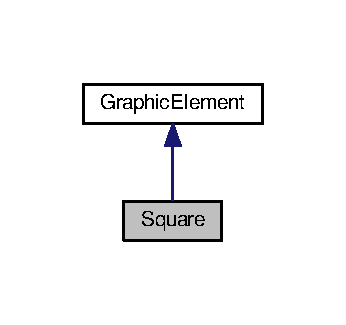
\includegraphics[width=166pt]{class_square__inherit__graph}
\end{center}
\end{figure}


Collaboration diagram for Square\-:
\nopagebreak
\begin{figure}[H]
\begin{center}
\leavevmode
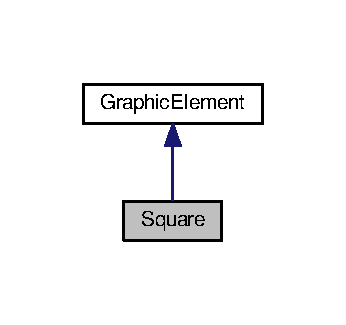
\includegraphics[width=166pt]{class_square__coll__graph}
\end{center}
\end{figure}
\subsection*{Public Member Functions}
\begin{DoxyCompactItemize}
\item 
void \hyperlink{class_square_a8f288729441c986e6fc37593c9c5346b}{create} () override
\item 
void \hyperlink{class_square_a90cb952f7266720cbd63513cd34a6fc3}{remove} () override
\end{DoxyCompactItemize}


\subsection{Member Function Documentation}
\hypertarget{class_square_a8f288729441c986e6fc37593c9c5346b}{\index{Square@{Square}!create@{create}}
\index{create@{create}!Square@{Square}}
\subsubsection[{create}]{\setlength{\rightskip}{0pt plus 5cm}void Square\-::create (
\begin{DoxyParamCaption}
{}
\end{DoxyParamCaption}
)\hspace{0.3cm}{\ttfamily [inline]}, {\ttfamily [override]}, {\ttfamily [virtual]}}}\label{class_square_a8f288729441c986e6fc37593c9c5346b}


Implements \hyperlink{class_graphic_element_ac059a330ae2aa071b80d4fc16f505a53}{Graphic\-Element}.

\hypertarget{class_square_a90cb952f7266720cbd63513cd34a6fc3}{\index{Square@{Square}!remove@{remove}}
\index{remove@{remove}!Square@{Square}}
\subsubsection[{remove}]{\setlength{\rightskip}{0pt plus 5cm}void Square\-::remove (
\begin{DoxyParamCaption}
{}
\end{DoxyParamCaption}
)\hspace{0.3cm}{\ttfamily [inline]}, {\ttfamily [override]}, {\ttfamily [virtual]}}}\label{class_square_a90cb952f7266720cbd63513cd34a6fc3}


Implements \hyperlink{class_graphic_element_a008cda41b56bfd1607067e478488405c}{Graphic\-Element}.



The documentation for this class was generated from the following file\-:\begin{DoxyCompactItemize}
\item 
\hyperlink{header_8h}{header.\-h}\end{DoxyCompactItemize}

\hypertarget{class_triangle}{\section{Triangle Class Reference}
\label{class_triangle}\index{Triangle@{Triangle}}
}


{\ttfamily \#include $<$header.\-h$>$}



Inheritance diagram for Triangle\-:
\nopagebreak
\begin{figure}[H]
\begin{center}
\leavevmode
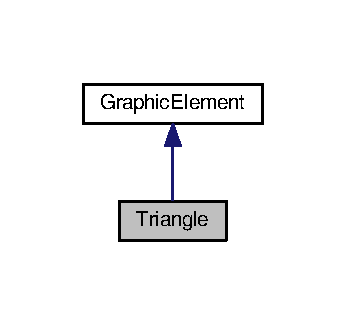
\includegraphics[width=166pt]{class_triangle__inherit__graph}
\end{center}
\end{figure}


Collaboration diagram for Triangle\-:
\nopagebreak
\begin{figure}[H]
\begin{center}
\leavevmode
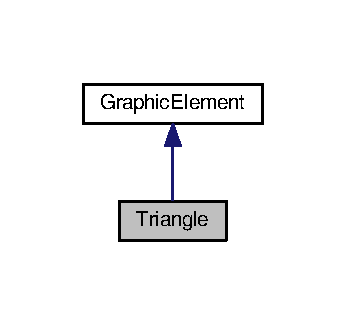
\includegraphics[width=166pt]{class_triangle__coll__graph}
\end{center}
\end{figure}
\subsection*{Public Member Functions}
\begin{DoxyCompactItemize}
\item 
void \hyperlink{class_triangle_a13b75277f5c2cd4991b599657b02692e}{create} () override
\item 
void \hyperlink{class_triangle_a38c4f7a80a0ef3dda7bc90652b510b46}{remove} () override
\end{DoxyCompactItemize}


\subsection{Member Function Documentation}
\hypertarget{class_triangle_a13b75277f5c2cd4991b599657b02692e}{\index{Triangle@{Triangle}!create@{create}}
\index{create@{create}!Triangle@{Triangle}}
\subsubsection[{create}]{\setlength{\rightskip}{0pt plus 5cm}void Triangle\-::create (
\begin{DoxyParamCaption}
{}
\end{DoxyParamCaption}
)\hspace{0.3cm}{\ttfamily [inline]}, {\ttfamily [override]}, {\ttfamily [virtual]}}}\label{class_triangle_a13b75277f5c2cd4991b599657b02692e}


Implements \hyperlink{class_graphic_element_ac059a330ae2aa071b80d4fc16f505a53}{Graphic\-Element}.

\hypertarget{class_triangle_a38c4f7a80a0ef3dda7bc90652b510b46}{\index{Triangle@{Triangle}!remove@{remove}}
\index{remove@{remove}!Triangle@{Triangle}}
\subsubsection[{remove}]{\setlength{\rightskip}{0pt plus 5cm}void Triangle\-::remove (
\begin{DoxyParamCaption}
{}
\end{DoxyParamCaption}
)\hspace{0.3cm}{\ttfamily [inline]}, {\ttfamily [override]}, {\ttfamily [virtual]}}}\label{class_triangle_a38c4f7a80a0ef3dda7bc90652b510b46}


Implements \hyperlink{class_graphic_element_a008cda41b56bfd1607067e478488405c}{Graphic\-Element}.



The documentation for this class was generated from the following file\-:\begin{DoxyCompactItemize}
\item 
\hyperlink{header_8h}{header.\-h}\end{DoxyCompactItemize}

\chapter{File Documentation}
\hypertarget{header_8h}{\section{header.\-h File Reference}
\label{header_8h}\index{header.\-h@{header.\-h}}
}
{\ttfamily \#include $<$iostream$>$}\\*
{\ttfamily \#include $<$string$>$}\\*
Include dependency graph for header.\-h\-:
\nopagebreak
\begin{figure}[H]
\begin{center}
\leavevmode
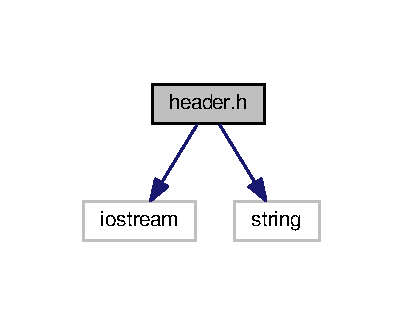
\includegraphics[width=193pt]{header_8h__incl}
\end{center}
\end{figure}
This graph shows which files directly or indirectly include this file\-:
\nopagebreak
\begin{figure}[H]
\begin{center}
\leavevmode
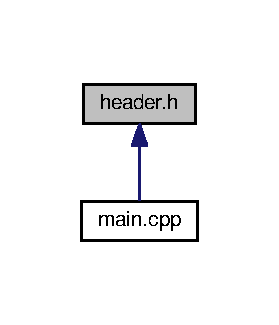
\includegraphics[width=134pt]{header_8h__dep__incl}
\end{center}
\end{figure}
\subsection*{Classes}
\begin{DoxyCompactItemize}
\item 
class \hyperlink{class_graphic_element}{Graphic\-Element}
\item 
class \hyperlink{class_line}{Line}
\item 
class \hyperlink{class_square}{Square}
\item 
class \hyperlink{class_triangle}{Triangle}
\item 
class \hyperlink{class_document}{Document}
\end{DoxyCompactItemize}

\hypertarget{main_8cpp}{\section{main.\-cpp File Reference}
\label{main_8cpp}\index{main.\-cpp@{main.\-cpp}}
}
{\ttfamily \#include \char`\"{}header.\-h\char`\"{}}\\*
{\ttfamily \#include $<$memory$>$}\\*
Include dependency graph for main.\-cpp\-:
\nopagebreak
\begin{figure}[H]
\begin{center}
\leavevmode
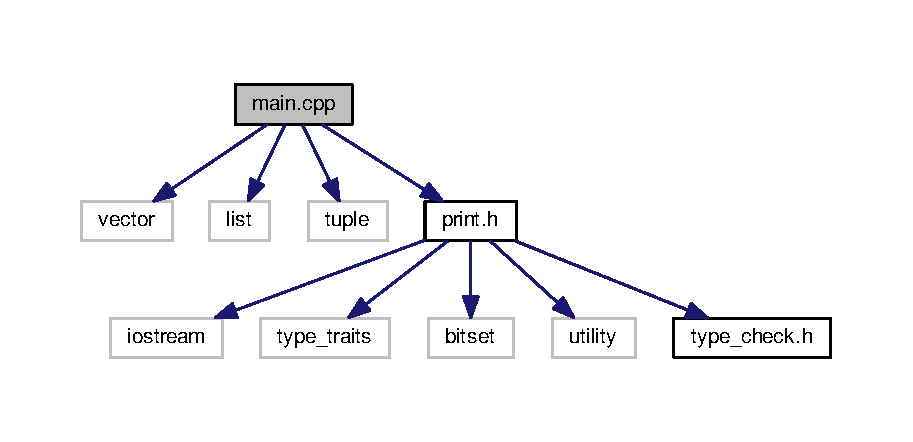
\includegraphics[width=237pt]{main_8cpp__incl}
\end{center}
\end{figure}
\subsection*{Classes}
\begin{DoxyCompactItemize}
\item 
class \hyperlink{class_graphic_editor}{Graphic\-Editor}
\end{DoxyCompactItemize}
\subsection*{Functions}
\begin{DoxyCompactItemize}
\item 
int \hyperlink{main_8cpp_ae66f6b31b5ad750f1fe042a706a4e3d4}{main} ()
\end{DoxyCompactItemize}


\subsection{Function Documentation}
\hypertarget{main_8cpp_ae66f6b31b5ad750f1fe042a706a4e3d4}{\index{main.\-cpp@{main.\-cpp}!main@{main}}
\index{main@{main}!main.cpp@{main.\-cpp}}
\subsubsection[{main}]{\setlength{\rightskip}{0pt plus 5cm}int main (
\begin{DoxyParamCaption}
{}
\end{DoxyParamCaption}
)}}\label{main_8cpp_ae66f6b31b5ad750f1fe042a706a4e3d4}

\hypertarget{version_8h}{\section{version.\-h File Reference}
\label{version_8h}\index{version.\-h@{version.\-h}}
}
\subsection*{Macros}
\begin{DoxyCompactItemize}
\item 
\#define \hyperlink{version_8h_a4a5fc96a4bdd7d68ed99ccce9ca2e77e}{P\-R\-O\-J\-E\-C\-T\-\_\-\-V\-E\-R\-S\-I\-O\-N\-\_\-\-P\-A\-T\-C\-H}~44
\end{DoxyCompactItemize}


\subsection{Macro Definition Documentation}
\hypertarget{version_8h_a4a5fc96a4bdd7d68ed99ccce9ca2e77e}{\index{version.\-h@{version.\-h}!P\-R\-O\-J\-E\-C\-T\-\_\-\-V\-E\-R\-S\-I\-O\-N\-\_\-\-P\-A\-T\-C\-H@{P\-R\-O\-J\-E\-C\-T\-\_\-\-V\-E\-R\-S\-I\-O\-N\-\_\-\-P\-A\-T\-C\-H}}
\index{P\-R\-O\-J\-E\-C\-T\-\_\-\-V\-E\-R\-S\-I\-O\-N\-\_\-\-P\-A\-T\-C\-H@{P\-R\-O\-J\-E\-C\-T\-\_\-\-V\-E\-R\-S\-I\-O\-N\-\_\-\-P\-A\-T\-C\-H}!version.h@{version.\-h}}
\subsubsection[{P\-R\-O\-J\-E\-C\-T\-\_\-\-V\-E\-R\-S\-I\-O\-N\-\_\-\-P\-A\-T\-C\-H}]{\setlength{\rightskip}{0pt plus 5cm}\#define P\-R\-O\-J\-E\-C\-T\-\_\-\-V\-E\-R\-S\-I\-O\-N\-\_\-\-P\-A\-T\-C\-H~44}}\label{version_8h_a4a5fc96a4bdd7d68ed99ccce9ca2e77e}

%--- End generated contents ---

% Index
\newpage
\phantomsection
\addcontentsline{toc}{chapter}{Index}
\printindex

\end{document}
